%%%%%%%%%%%%%%%%%%%%%%%%%%%%%%%%%%%
\subsection{Purity Monitors} 
\label{sec:fdsp-slow-cryo-purity-mon}
%Laura, Jianming
A fundamental requirement of a LAr TPC is to make ionization electrons drift over long distances in liquid argon. Part of the charge is inevitably lost due to the presence of electronegative impurities in the liquid. To keep such loss to a minimum, purifying the liquid argon during operation is essential, as it is the monitoring of impurities.

Residual Gas Analyzers are an obvious choice when analyzing gas argon and can be exploited for the monitoring of the gas in the ullage of the tank. Unfortunately, commercially available mass spectrometers have a detection limit of $\sim$10\,ppb, whereas DUNE requires a sensitivity down to the ppt level. This gives us a case to construct small, ``portable'' devices, called ``purity monitors'', to monitor purity in all the phases of operations, guaranteeing successful commissioning and meeting the requirement to measure position-dependent purity necessary to achieve DUNE's physics goal. 
%Purity monitors also have the potential to be developed as a calibration tool that provides high precision and real-time electron lifetime measurements for wire-by-wire detector calibration. 

Purity monitors will be placed inside the vessel, as well as outside the cryostat \textcolor{red}{before and after} the recirculation system.

Purity monitors have already been successfully employed in the ICARUS detector and in the 35-ton prototype detector at Fermilab. The ProtoDUNE Single-Phase and Dual-Phase detectors also employ purity monitors. A similar design to the ones used in the ProtoDUNEs will be exploited in the DUNE FD.

\subsubsection{Physics and Simulation}
% Andrew, Jianming
A purity monitor (PrM) is a miniature TPC which directly measures the electron lifetime, $\tau$, in the liquid argon and does not depend on the LAr TPC high voltage, electronics, and data acquisition. The concentration of electronegative impurities such as $O_2$ and $H_2O$(which the electron lifetime mosty depends on) is inversely proportional to the electron lifetime according to the following formula [CITE Bakale Sowada Schmidt, The Journal of Physical Chemistry, Vol. 80,No. 23, 7976]:

$$\tau = \sum_i \frac{1}{k_i [S_i]}$$

where the sum runs over all species of impurities in the liquid; $\tau$ is in s; $k_i$ is the electron attachment coefficient rate specific to the impurity in units of $l (mol s)^-1$; and $[S_i]$ is the concentration of the specific impurity in units of $mol/l$. The electron attachment rate is a function of electric field, but this field dependence is not significant for the range of LArTPC operation (electric field of $\sim$ 500V/cm), as shown in Figure~\ref{fig:ks}.

\begin{figure}[h]
\centering
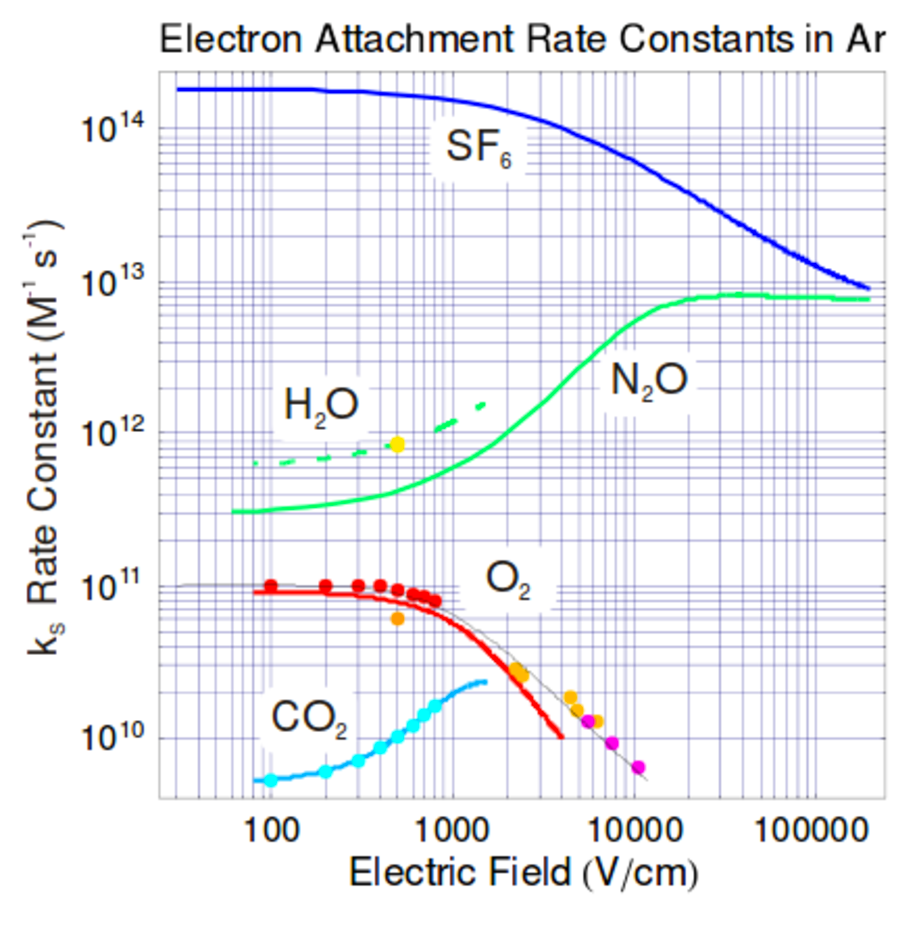
\includegraphics[height=6cm]{PrMon_ks.pdf}
\caption{Electron attachment rate ($k_s$) as a function of electric field for several contaminants in a LAr TPC.}\label{fig:ks}
\end{figure}

Assuming all impurities affecting the electron lifetime are of type $O_2$, the electron lifetime may be converted into ``ppb oxygen equivalent":

$$ \O_2 [ppb] = \frac{300 [ppb \mu]}{\tau [\mu s]}$$

Depending on their length and the electric field operated at, purity monitors can be sensitive to tens of ppt oxygen equivalent. 

For the single-phase DUNE far detector module the drift distance is 3.6 m. For the dual-phase DUNE far detector module the maximum drift distance is 12 m, and the requirement for the electron lifetime is even higher. 

%The loss of electrons during drift is primarily caused by the electron attachment to the electro-negative impurities, such as oxygen and water in the liquid argon. 

The electron loss can be parameterized as

$$N(t) = N(0)e^{-t/\tau},$$

where $N(0)$ is the number of electrons generated by ionization, $N(t)$ is the number of electrons after drift time $t$, and $\tau$ is the electron lifetime. 

%The relation between the electron lifetime and the impurity can be expressed as

%$$\tau = \frac{1}{k_s\times n_s},$$

%where $k_s$ is the electron attachment rate and $n_s$ is the concentration of a certain type of impurity. The electron attachment rate is a function of electric field, but this field dependence is not significant for the range of LArTPC operation (electric field of $\sim$ 500V/cm), as shown in Figure~\ref{fig:ks}.

%\begin{figure}[h]
%\centering
%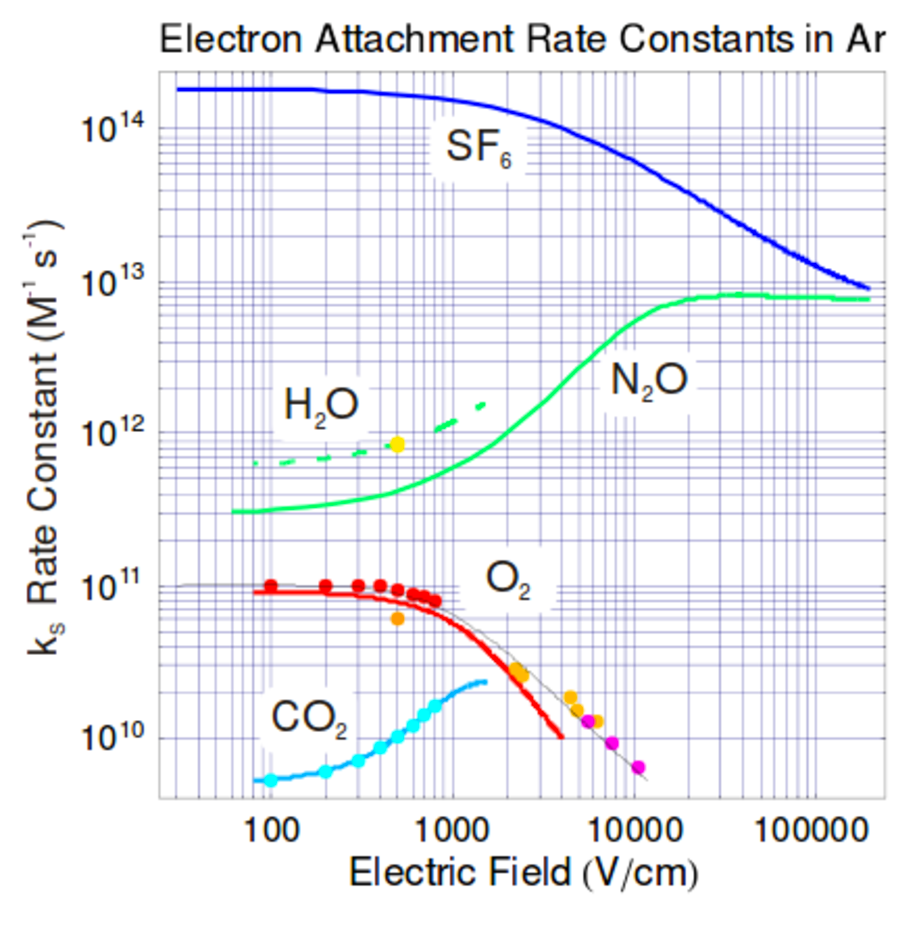
\includegraphics[height=6cm]{PrMon_ks.pdf}
%\caption{Electron attachment rate ($k_s$) as a function of electric field for several contaminants in a LAr TPC.}\label{fig:ks}
%\end{figure}

For the single-phase DUNE far detector module, the drift distance is 3.6 m and the electric field is 500 V/cm, and the maximum drift time is about 2.4 ms. If we want to keep the signal attenuation, [N(0)-N(t)]/N(0), to be less than  20\% over the drift distance, the necessary electron lifetime is $2.4/[-\ln(0.8)] \simeq 11 $ms, and the corresponding liquid argon purity requirement is about 30 parts per trillion (ppt). For the dual-phase DUNE far detector module, the maximum drift distance is 12 m and the requirements of the electron lifetime and purity are much higher. Therefore, purity monitoring is essential for successful operation of a LAr TPC. Furthermore, to understand the LAr TPC detector response and performance, precise measurements of electron lifetime in liquid argon are very important.

The DUNE 35-ton prototype detector at Fermilab was instrumented with four purity monitors. The data taken with them during the first part of the second phase is shown in Fig.~\ref{fig-35t-prm} and clearly shows the ability to measure the electron lifetime between 100 $\mu$s and 3.5 ms.  Because the scale of the DUNE detector (and especially the DUNE far detectors) are so much larger, there is a significant danger that sudden changes in the purity of the liquid argon being injected back into the cryostat might go unnoticed. If this were to occur for too long it would cause irreversible contamination to the liquid argon and terminate useful data taking.  Having purity monitors continuously monitoring the detector, placed in strategic places and then used as an interlock, it could be possible to salvage the overall purity of the detector and maintain the ability to take good data. An irreversible contamination cannot be tolerated in the DUNE far detectors, and so strategically placed purity monitors must be implemented to mitigate this risk. 

%A purity monitor's basic design is based on those used by the ICARUS and LAPD experiments~\cite{Carugno:1990kd, Adamowski:2014daa} (Figure~\ref{fig:PrMon}). It is a double-gridded ion chamber immersed in the liquid argon volume. It measures the electron drift lifetime between its anode and cathode. The electrons are generated by the purity monitor's UV-illuminated gold photocathode. The UV is generated by a xenon flash lamp. The electron lifetime in liquid argon is inversely proportional to the electronegative impurity concentration. The fraction of electrons generated at the cathode that arrive at the anode ($Q_A/Q_C$) after the electron drift time $t$ is a measure of the electron lifetime $\tau$: $Q_A/Q_C=e^{-t/\tau}$. 


\begin{figure}[t!]
\begin{center}
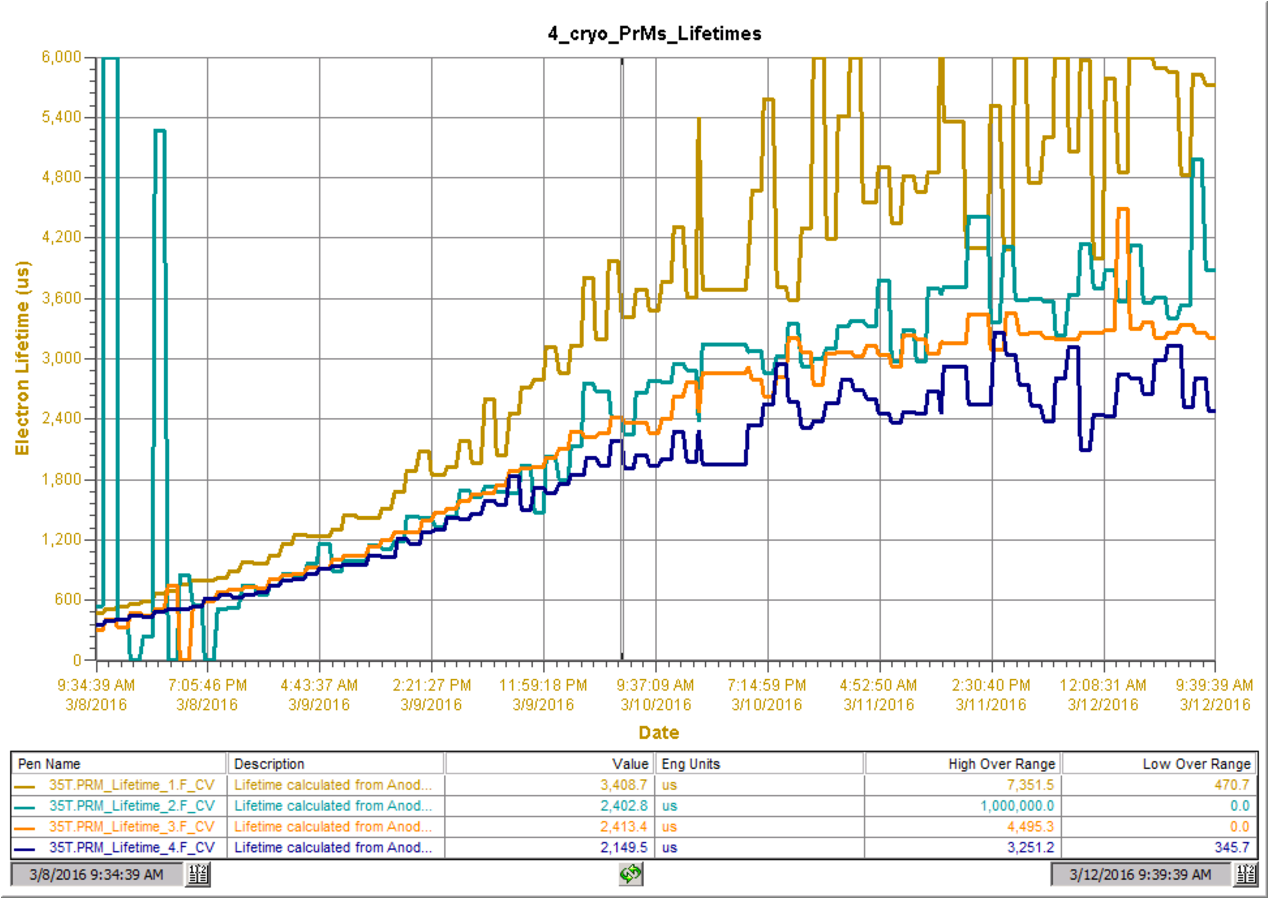
\includegraphics[width=10cm]{PrMon_35t-PrM.pdf}
\caption{The measured electron lifetimes in the four purity monitors as a function of time at Fermilab 35T prototype.} \label{fig-35t-prm}
\end{center}
\end{figure}


\subsubsection{Purity Monitor Design}
%Laura, Jianming

%THIS WAS ALREADY SAID. The purity (electron lifetime) of liquid argon inside a large detector needs to be continuously monitored by purity monitors strategically placed within the detector cryostat. 
%IF YOU HAVE MIP PARTICLES LIKE MUONS... NOT TRUE WHEN YOU ARE UNDERGROUND. ALSO, WE HAVE SEEN IN THE 311 THAT MUONS DO NOT DEPOSIT THE EXACT SAME AMOUNT OF ENERGY ACROSS THE TRACK (1 M DRIFT!) While the LAr TPC itself can measure the purity of the liquid argon based on the drift electron lifetime, this can only be done once a certain level of purity has been achieved, and until then it may be unclear what the level of purity is and if conditions in the detector are becoming better or worse. 
%NOT SURE WHERE TO PUT THIS In addition, because a purity monitor can measure purity with high precision at a specific point, it is possible to determine the gradient of purity with properly deployed purity monitors.

The basic design of a purity monitor is based on those used by the ICARUS experiment (Figure~\ref{fig:prm}). It is a double-gridded ion chamber immersed in the liquid argon volume. 
The purity monitor consists of four parallel, circular electrodes: a photocathode held in place by a groove in a stainless-steel disk, two grids (cathode and anode), and a stainless-steel anode plate. 
%The purity monitor consists of four parallel, circular electrodes: a disk holding a photocathode, two grid rings (anode and cathode), and an anode disk. 
The cathode grid is at ground potential. The cathode, anode grid, and anode are electrically accessible via modified vacuum grade high voltage feedthroughs. 
The anode grid and the field shaping rings are connected to the cathode grid by an internal chain of 50 M$\Omega$ resistors to ensure the uniformity of the electric fields in the drift regions. 
A stainless mesh cylinder is used as a Faraday cage to isolate the purity monitor from electrostatic b b backgrounds. The purity monitor measures the electron drift lifetime between its anode and cathode. The electrons are generated by the purity monitor's UV-illuminated gold photocathode via photoelectric effect. As the electron lifetime in liquid argon is inversely proportional to the electronegative impurity concentration, the fraction of electrons generated at the cathode that arrive at the anode ($Q_A/Q_C$) after the electron drift time $t$ is a measure of the electron lifetime $\tau$: $Q_A/Q_C=e^{-t/\tau}$.
%THIS FORMULA IS ONLY APPRIXIMATE, CORRECT FORMULA IS: Q_A/Q_C = \frac{T_C \sinh(T_A/2\tau))}{T_A \sinh(T_C/2\tau)} \exp \left(-\frac{T_D+\frac{T_A+T_C}{2}}{\tau} \right)

\begin{figure}[h]
\centering
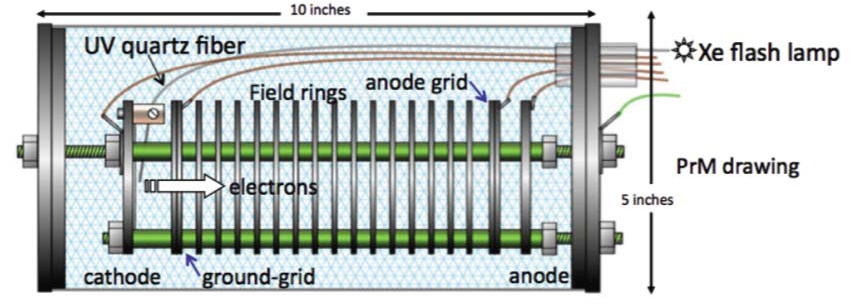
\includegraphics[height=3cm]{PrMon_prm.pdf}
\caption{Schematic diagram of the basic purity monitor design.}\label{fig:prm}
\end{figure}

The photocathode that produces the photoelectrons is an aluminum plate coated with 50 $\rm\r{A}$ of titanium and 1000 $\rm\r{A}$ of gold and attached to the cathode disk. A xenon flash lamp is used as the light source in the baseline design, although this should be replaced by a more reliable and possibly submersible light source in the future. The UV output of the lamp is quite good around $\lambda$ = 225 nm, which is close to the work function of gold (4.9-5.1 eV). Several UV quartz fibers are used to carry the Xe UV light into the cryostat to illuminate the gold photocathode. 
Another quartz fiber is used to deliver the light into a properly biased photodiode outside of the cryostat to provide the trigger signal when the lamp flashes. There is also an option for upgrading the light source to an LED version.
%REALLY?

\subsubsection{Electronis, DAQ and Slow Controls Interfacing}
%Jianming
Purity Monitor electronics and DAQ system consist of front-end electronics, waveform digitizers, and a DAQ PC.   The block diagram of the system is shown in Fig~\ref{fig:diagram}. 

The base design of the front-end electronics is the one used in purity monitors at 35T, LBNF, and MicroBOONE. It is composed of an HV filter circuit and a charge amplifier circuit. The cathode and anode signals are fed into two charge amplifiers contained within the purity monitor electronics module. This electronics module includes a filter circuit and an amplifier circuit that are shielded by copper plates, so the signal and high voltage can be carried on the same cable and decoupled inside the purity monitor electronics module. The amplified outputs of the anode and cathode will be measured with a digitizer that interfaces with either a DAQ PC. The shields of the signal and HV cable connected to the grounding point of the cryostat are separated from the electronic ground with a resistor and a capacitor connected in parallel. The amplified outputs are transmitted to an AlazarTech ATS310 waveform digitizer, which features two input channels with a 12-bit resolution. Each channel is capable of sampling a signal at a rate of 20~MS/s to 1~kS/s and storing up to 8 million samples in a memory. The digitizer is used per purity monitor and interfaces with a DAQ PC across the PCI bus.

\begin{figure}[h]
	\centering
	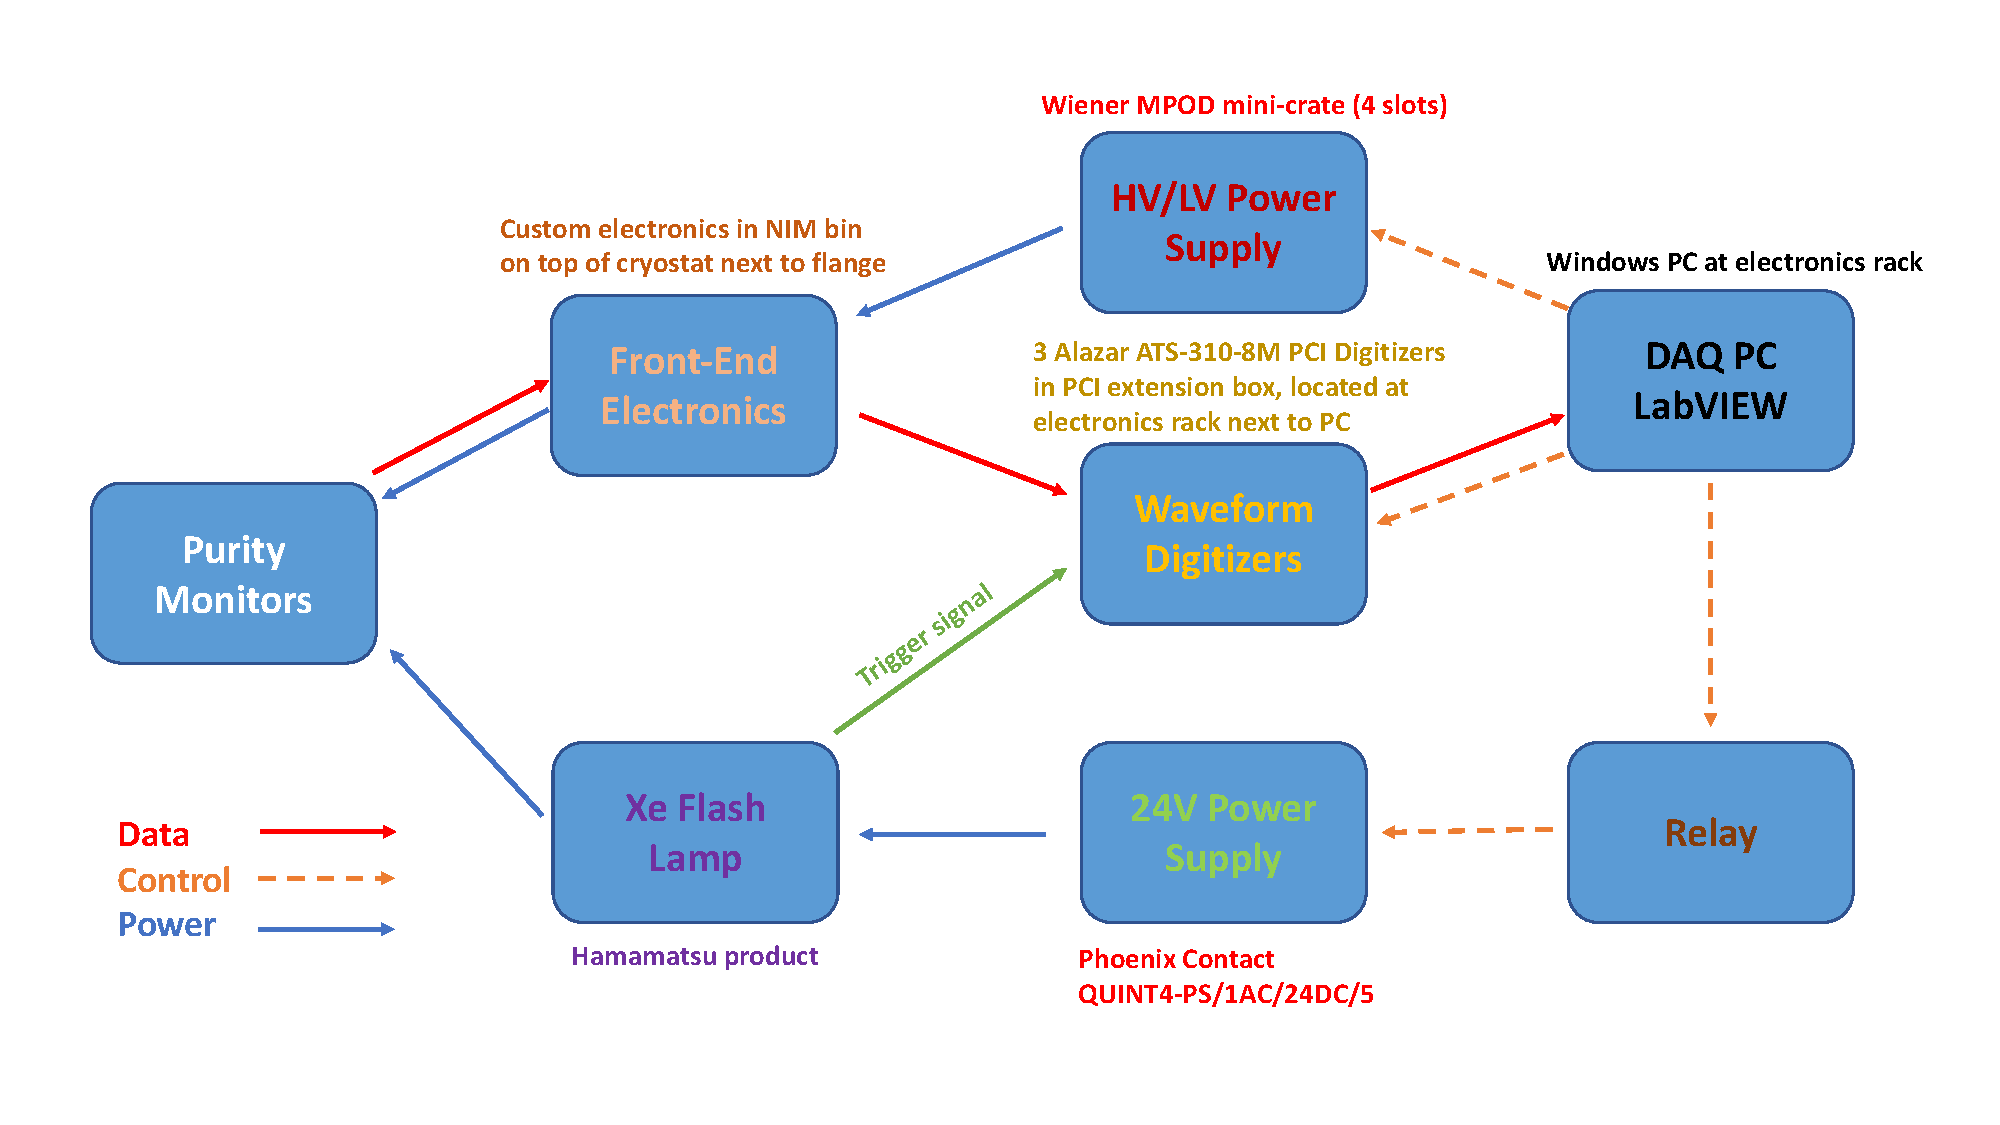
\includegraphics[width=0.8\textwidth]{PrMon_BlockDiagram.pdf}
	\caption{Block diagram of Purity Monitor system}
	\label{fig:diagram}
\end{figure}

A custom LabVIEW application running in the DAQ PC is developed and consists of two functions: controlling the digitizers and the power supplies, and monitoring the signals and key parameters. The application configures the digitizers to set a sampling rate, a number of storing waveforms in the memory, pre-trigger data, and a trigger mode. A signal from the Xe flash lamp is directly fed into the digitizer as an external trigger to initiate data acquisition. The LabVIEW application automatically turns on the Xe flash lamp by controlling the relay with start and turns it off when ends. The waveforms stored in the digitizers are transferred to the DAQ PC and used to obtain averaged waveforms to reduce the electronic noise present in waveforms. The baseline is estimated by using the pre-trigger data and subtracted from the waveforms to measure peak voltages of the cathode and anode signals. These processes are performed in real time within the application and are used to estimate electron lifetime. The application continuously displays the waveforms and important parameters, such as electron lifetime, peak voltages, and drift time of electrons in the purity monitors, and also shows these parameters over time. This allows one to validate the impurity of LAr and see effects that may not spot on an event by event basis. Instead of storing the measured parameters, the waveforms and the digitizer configurations are recorded in binary form for offline analysis. ISEG HV modules with WIENER MPOD Mini crate are used to supply negative and positive voltages to the cathode and the anode, respectively. The LabVIEW application will control and monitor the HV systems through an Ethernet interface.  

The Xe flash lamp and the front-end electronics will be installed close to the purity monitor flange to reduce light loss in an optical fiber and signal loss. Other pieces of equipment will be mounted in a DCS rack. They distribute powers to the flash lamp and the front-end electronics and collect data from the electronics. The DCS system will communicate with the purity monitor DAQ software and have the control of HV and LV of the purity monitor system. 

The electronics of Purity Monitors may induce noise in TPC electronics which is caused by the current surge in the discharging process of the main capacitor of the purity monitor xenon light source when producing a flash.  The light source for the purity monitor system will produce a lot of UV light in the detector which could potentially interfere with physics measurements and damage the Photon Detector System. To solve these problems, a software will be developed for a light source triggering mechanism to prevent the PrM flash lamp from flashing during TPC and photon detector data taking. The purity monitor will also send signals to TPC and photodetectors to veto any TPC/photon signals during Purity monitor measurements. In addition, we will make faraday cage to the ground and shield the light source.

%\begin{dunefigure}[Purity Monitor]{fig:PrMon}
%  {Overall design of the individual purity monitors devices which are immersed into the LAr.}
%  \includegraphics[width=0.3\textwidth]{PrMon.pdf}%
%\end{dunefigure}


\subsubsection{Production and Assembly}
\label{sec:PrMon-Production-Assembly}
%Andrew
Production of the individual purity monitors and the assembly of them into the string that will be placed into the DUNE-FD cryostat will follow the same methodology that is being developed for DUNE.  Each of the individual monitors will be fabricated, assembled and then tested in a smaller test stand.  After confirming that each of the individual purity monitors operates at the required performance, they would be assembled together via the support tubes used to mount the system to the inside of the cryostat such that three purity monitors are grouped together to form a "string" of purity monitors, as shown in Fig.~\ref{fig:PrMon-SystemString}.  The assembly of the individual purity monitors into the string would follow the steps laid out in the first 5 panels of Fig.~\ref{fig:PrMon-Assembly}.  

\begin{dunefigure}[Purity Monitor String]{fig:PrMon-SystemString}
  {Design of the purity monitor string that will contain three purity monitors.}
  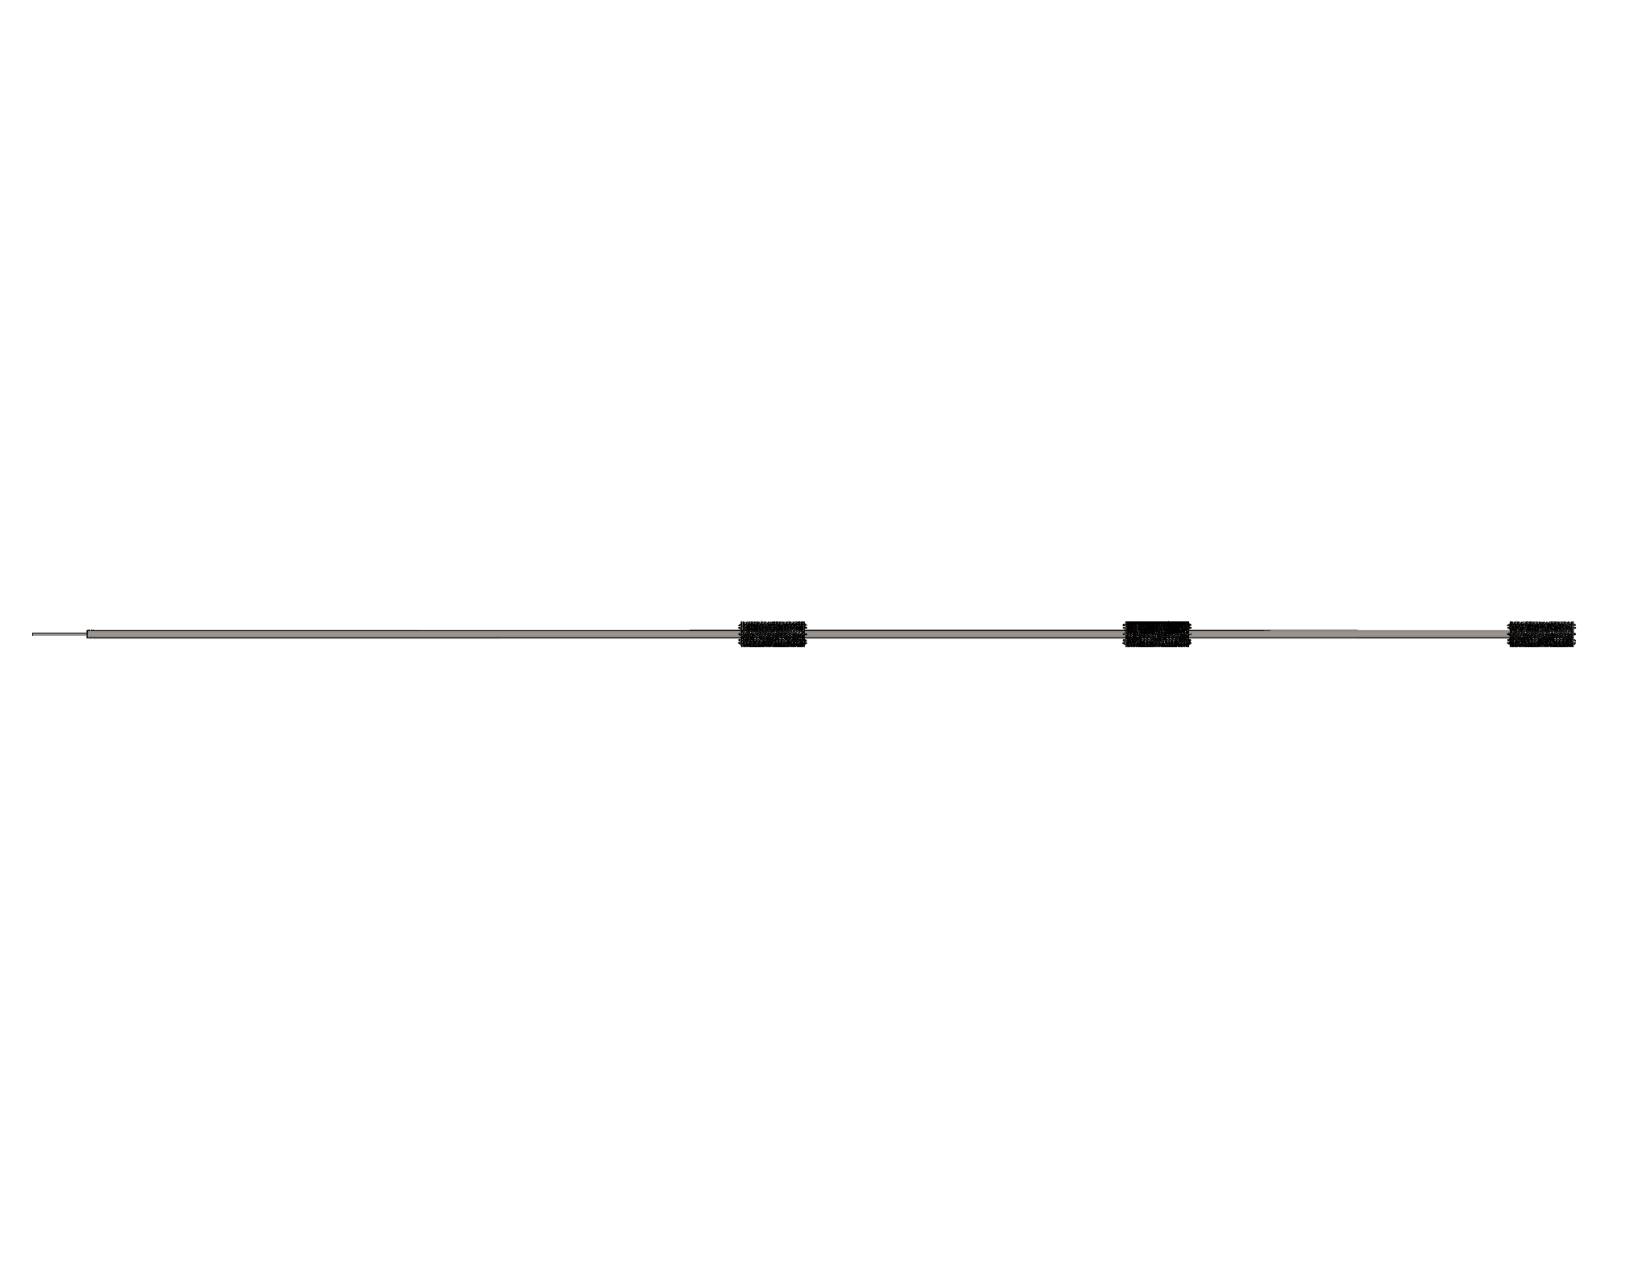
\includegraphics[width=\textwidth]{PrMon-SystemString.pdf}
\end{dunefigure}

\begin{dunefigure}[Purity Monitor String Assembly]{fig:PrMon-Assembly}
  {Assembly sequence of the purity monitors.}
  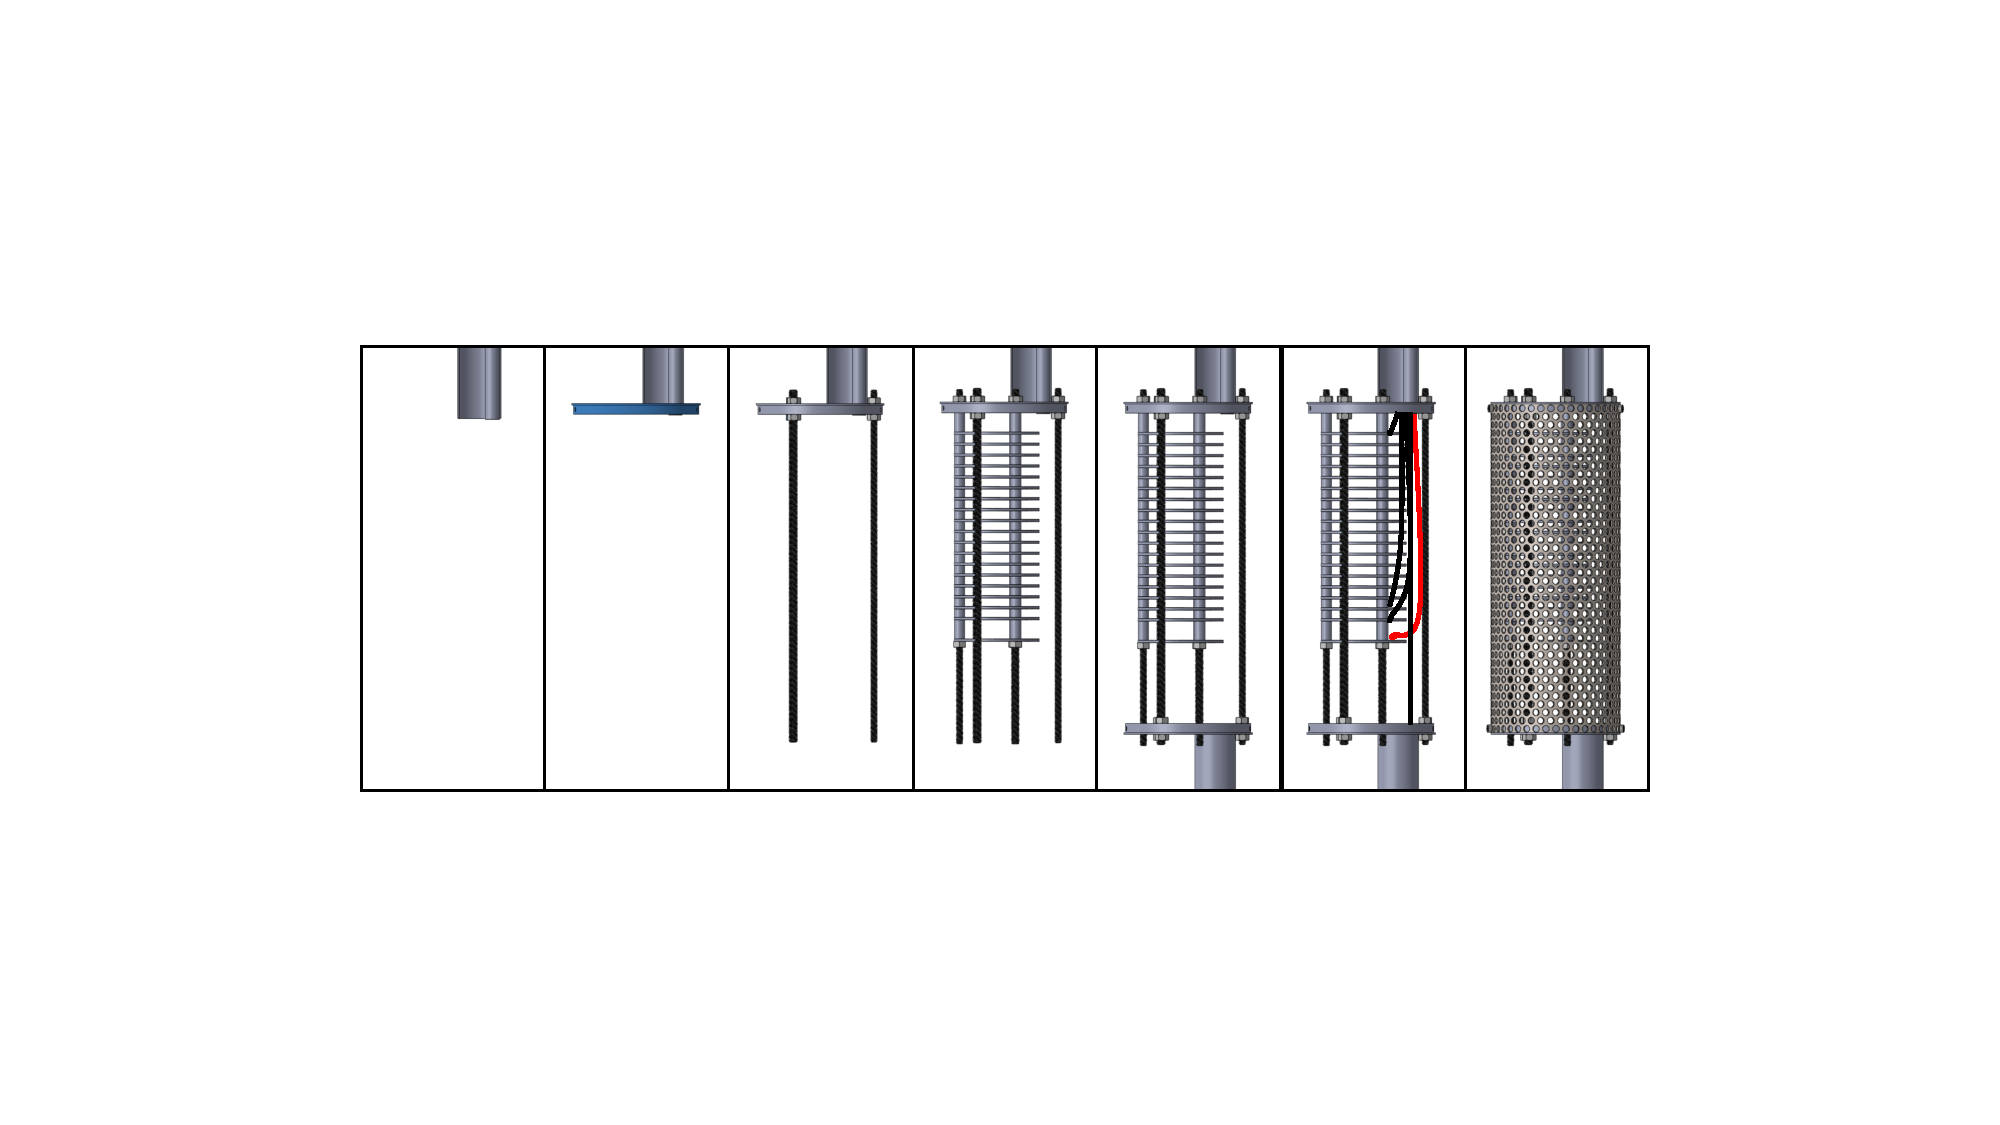
\includegraphics[width=\textwidth]{PrMon-Assembly.pdf}
\end{dunefigure}


\subsubsection{Installation, Integration and Commissioning}
\label{sec:PrMon-Install-Integrate-Commission}
%Andrew
The purity monitor system will be built in a modular way, such that is can be assembled outside of DUNE-FD cryostat.  The assembly of the purity monitors themselves would occur outside of the cryostat and would include everything described in Sec.~\ref{sec:PrMon-Production-Assembly}.  The installation of the purity monitor system can then be carried out with the least number of steps inside the cryostat.  The assembly itself would come into the cryostat with the three individual purity monitors mounted to the support tubes and no HV cables or optical fibers installed yet.  The support tube at the top and bottom of the assembly would then be mounted to the brackets inside the cryostat that could be attached to the cables trays and/or the detector support structure.  In parallel to this work, the front-end electronics and light source can be installed on the top of the cryostat, along with the installation of the electronics and power supplies into the electronics rack.  

Integration would begin by running the HV cables and optical fibers to the purity monitors, coming from the top of the cryostat.  The HV cables would be attached to the HV feedthroughs with enough length to reach each of the respective purity monitors.  The cables would be run through the port reserved for the purity monitor system, along cable trays inside the cryostat until they reach the purity monitor system, and would then be terminated through the support tube down to each of the purity monitors.  Each purity monitor will have three HV cables that connect it to the feedthrough, and then along to the front-end electronics.  The optical fibers would then be run through the special optical fiber feedthrough, into the cryostat, and would be guided to the purity monitor system either using the cables trays or guide tubes.  Which ever solution is adopted for running the optical fibers from the feedthrough to the purity monitor system, it should protect the fibers from accidental breakage during the remainder of the detector and instrumentation installation process.  The optical fibers would then be run inside of the purity monitor support tube and to the respective purity monitors terminating them at the photocathode of each, protecting them from breakage near the purity monitor system itself.

Integration would continue with the connection of the HV cables between the feedthrough and the system front-end electronics, and then optical fibers to the light source.  The cables connecting the front-end electronics and the light source to the electronics rack would also be run and connected at this point.  This would allow for the system to be turned on and the software to begin testing the various components and connections.  Once it was confirmed that all connections had been successfully made, the integration to the slow controls system would be made, first by establishing communications between the two systems and then transferring mach data between them to ensure successful exchange of important system parameters and measurements.  

Commissioning of the purity monitor system would officially be done once the cryostat had been purged and a gaseous argon atmosphere was present.  At this point the HV for the purity monitors could be ramped up without the fear of discharge through the air, and the light source the turned on.  Although the drift electron lifetime in the gaseous argon would be very large and therefore not really measurable with the purity monitors themselves, the signal strength at both the cathode and anode would give a good indication of how well the light source is generating drift electrons from the photocathode and that they are successfully drifted to the anode by looking at the signal strength at the anode and comparing it to that of the cathode.


%\subsubsection{Quality Control}
%This subsubsection has been moved to the official Quality Control subsection and the text has already been provided by Andrew, please double check it and confirm that is it fine and feel free to recommend suggestions for improvement.


